\documentclass{article}
\usepackage{blindtext}
\usepackage[utf8]{inputenc}
\usepackage[spanish, mexico]{babel}

\usepackage{graphicx}  
\usepackage{listings}

\usepackage{listings}
\usepackage{xcolor}
\usepackage{multirow}
\usepackage{array}
\usepackage{amsmath}
\usepackage[ruled,vlined]{algorithm2e}

\definecolor{codegreen}{rgb}{0,0.6,0}
\definecolor{codegray}{rgb}{0.5,0.5,0.5}
\definecolor{codepurple}{rgb}{0.58,0,0.82}
\definecolor{backcolour}{rgb}{0.95,0.95,0.92}

\lstdefinestyle{mystyle}{
    backgroundcolor=\color{backcolour},   
    commentstyle=\color{codegreen},
    keywordstyle=\color{magenta},
    numberstyle=\tiny\color{codegray},
    stringstyle=\color{codepurple},
    basicstyle=\ttfamily\footnotesize,
    breakatwhitespace=false,         
    breaklines=true,                 
    captionpos=b,                    
    keepspaces=true,                 
    numbers=left,                    
    numbersep=5pt,                  
    showspaces=false,                
    showstringspaces=false,
    showtabs=false,                  
    tabsize=2
}

\lstset{style=mystyle}

\title{Sistema de detección y reconocimiento de rostros con el uso de HOG }
\author{Pedro Damián Cruz Santiago} 
\date{February 2021}

\begin{document}
\maketitle

\begin{abstract}
La mayoría de los métodos de detección de objetos funcionan aplicando un clasificador binario a las subventanas de una imagen, a continuación se aplica el método de non maximun supression para eliminan las detecciones en subventanas superpuestas. La generación de subventanas y la aplicación del clasificador sobre ellas puede pensarse como la aplicación de la misma tarea sobre diferentes datos es decir se identifica un paralelismos de datos. En el presente trabajo se presenta un a documentación sobre las diferentes etapas de la identificación de objetos en una imagen, se presentará una estrategía numérica para abordar el problema de detección de rostros humanos y por útimo se desarrollará una propuesta de solución en el lenguaje de programación python con el uso de paquetes auxiliares en el menejo de arreglos y el uso de clasificadores lineales.


\end{abstract}

\section*{Introducción}
\subsection*{Visión por computadora}
La visión por computadora es un tema o área de investigación  dentro de la inteligencia artificial en específico "machine leaarning", que trata de emular la capacidad del ser humano de  "ver" mediante la interpretación de una imagen o una secuencia de éstas como lo es un
vídeo), y reconocer los diversos objetos en el ambiente y su posición en el espacio.  Podemos mencionar 2 enfoques de la visión por computadora:
\begin{itemize}
  \item Procesamiento de imágenes.
  \item Visión computaciones.
\end{itemize}
El objetivo del primero es mejorar la calidad de las imágenes para su posterior utilización o interpretación, mientras que el objetivo del segundo es extraer característicos de una imagen para su descripción e interpretación por la computadora. 
En la figura \ref{fig:lena-contraste} se muestra un ejemplo de procesamiento de imágenes. La tarea a realizar es \textit{mejorar} la imagen de entrada, la imagen de salida es la \textit{misma} pero con mejor calidad o \textit{más útil}. La figura \ref{fig:placas} muestra la diferencia entre el procesamiento de imágenes y visión poor computadora; la imagen muestra diferentes etapas de un proceso a la que fue sometida una imagen para extraer descripciones importantes, la salida o resultado de este procesamiento se complementa con sistema de reconocimiento de patones, es decir \textit{saber} qué letras y números contiene la placa\cite{placas}.

\begin{figure}[ht]
\centering
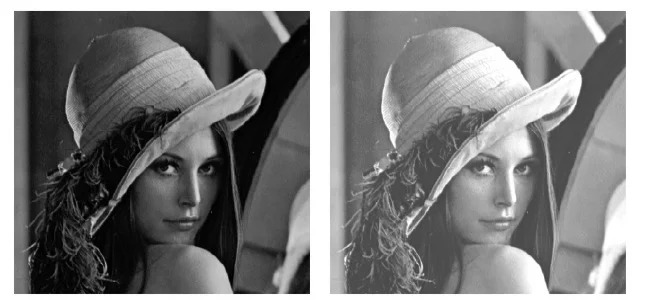
\includegraphics[width=.75\textwidth]{lena-contraste.jpg}
\caption{Aumento de contraste: En el lado derecho se observa la misma imagen \textit{mejorada} de la izquierda después de mejorar el contraste o ecualización del histograma de la escala de grises.}
\label{fig:lena-contraste}
\end{figure}

\begin{figure}[ht]
\centering
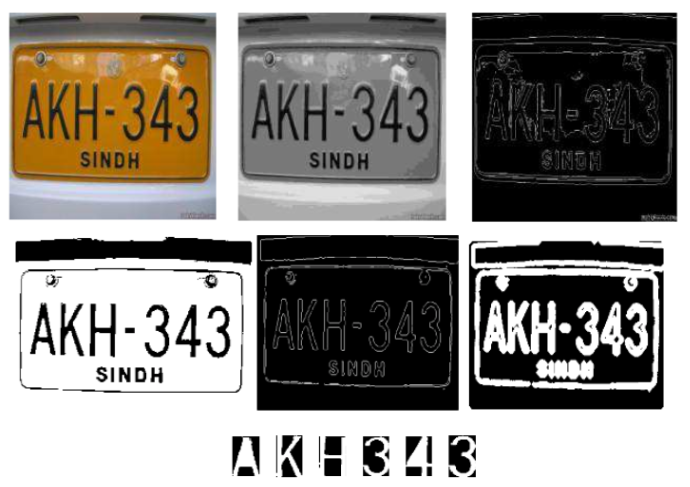
\includegraphics[width=0.75\textwidth]{placas-viz.png}
\caption{Extracción de información: La identificación de una placa a partir de una fotografía consiste en aplicar varios cálculos a cada píxel de tal forma que la computadora sea capaz de comparar cada elemento con un patrón. Imagen tomada de \cite{placas} }
\label{fig:placas}
\end{figure}
\subsection*{Detección de objetos}
La detección de objetos dentro del ámbito de la visión por computadora consiste en el problema de detectar cierta clase de objetos como personas, automóviles, rostros humanos, en una imagen. Estas clases de objetos pueden aparecer en una imagen a diferentes tamaños, colores, iluminación, en diferentes ángulos o poses, lo que dificulta su detección. El reto es entonces desarrollar un algoritmo de detección que sea capaz de tratar con esas variaciones del objeto a detectar. Hay varias propuestas de algoritmos \textit{invariantes} abordando la detección del objeto completo \cite{dalal-triggs} o compuesto por varias partes rígidas o flexibles \cite{hog-parts1} \cite{hog-parts2}. Para la detección del objeto estos trabajos \textit{escanean} la imagen con la ayuda de una rectángulo de tamaño fijo llamado ventana, el tamaño de la ventana deberá ser proporcional al objeto que se quiere detectar por ejemplo \cite{dalal-triggs} reportan un tamaño de 128x64 píxeles para la detección de humanos, mientras que \cite{hog-parts1} \cite{hog-parts2} utilizan diferentes tamaños de ventana para la detección del objeto y sus partes. Cada ubicación de la ventana en la imagen es un posible candidato para la detección del objeto, se obtiene su  descriptor \textbf{HOG} y se clasifica con la ayuda de un \textbf{SVM} para determinar si contiene o no el objeto de interés. 
\subsection*{Detección y reconocimiento facial}
La detección facial es el proceso en el que el software determina, mediante algoritmos, si hay rostros humanos en una foto o vídeo. No determina la identidad de una persona, tan solo determina si hay alguna cara. Por otro lado el sistema de reconocimiento facial es una aplicación que se encarga de identificar automáticamente a una persona, el cual realiza un  análisis  de  las  características  faciales  del  usuario adquiridas mediante una imagen  y comparándolas con una base de datos. 

Podemos considerar la detección facial o de rostros humanos como un caso específico de la detección de objetos que se vuelve un reto para la visión por computadora debido a que rostro humano no es objeto rígido (gestos o expresiones), puede aparecer en diferentes tonalidades de color de piel, parcialmente, con accesorios como anteojos o bigote, por mencionar algunas \cite{caras-resumen}. 
En 2001 se presento un trabajo que permitió por primera vez la detección y seguimiento de rostros en un vídeo \cite{viola-jones} pero con las desventajas de trabajar en imágenes solo en escala de grises y ser susceptible a fallas si la imagen a procesar contenía niveles de brillo muy altos o muy bajos, estas limitantes motivaron al desarrollo de otros algoritmos invariantes a éstas como el uso de HOG descriptor invariante al color y luminosidad o brillo de la imagen.
\subsection*{HOG: Histrograma de gradientes orientados}
Los  algoritmos  de  procesamiento  buscan  extraer  características  al  convertir  una  imagen  de  tamaño  fijo  en  un  vector.  Esta  transformación  sirve  para  detectar  patrones.  

Es bastante común que una imagen de entrada posea demasiada información adicional que no es necesaria para la detección de una clase de objeto, por ejemplo un rostro humano. Por lo tanto, el primer paso en proceso de la detección de objetos  es  simplificar  la  imagen  extrayendo  la  información  importante contenida en esta y dejando de lado el resto. Este paso se llama extracción de características el cual consiste en tranformar una imagen de tamaño fijo en un vector de longitud fija, el histograma  de  gradientes  orientados \textbf{HOG} es uno de los más utilizados. En la tabla \ref{table:1} se muestran valores con mejores resultados utilizados para la construcción de vector \textbf{HOG} \cite{dalal-triggs}. \\

\begin{figure}
\centering
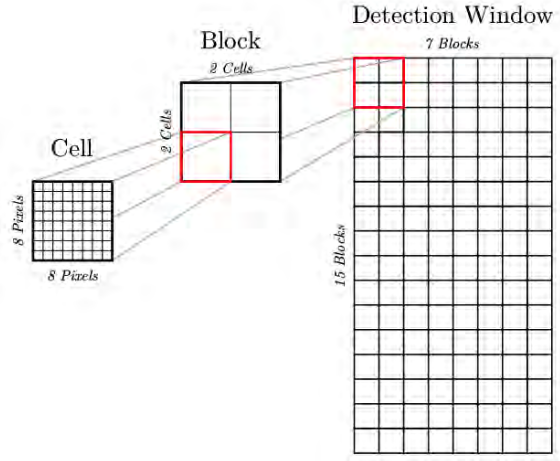
\includegraphics[width=5cm]{celda-bloque-ventana.png}
\caption{Divición de la ventana en bloques y celdas para el calculo del HOG}
\label{fig:celda-bloque-venana}
\end{figure}

Podemos resumir el algoritmo para la detección de objetos de la figura \ref{fig:hog} de la siguente forma: La imagen se divide en pequeñas regiones conectadas llamadas celdas, y para los píxeles dentro de cada celda, se construye un histograma gradientes orientados. El descriptor o vector es la concatenación de estos histogramas. Para mejorar la precisión, los histogramas locales se pueden normalizar por contraste calculando una medida de la intensidad en una región más grande de la imagen, llamada bloque, y luego usando este valor para normalizar todas las celdas dentro del bloque. Esta normalización da como resultado una mejor invariancia a los cambios de iluminación y sombreado. Por último se concatenan los vectores de todos los bloques y el vector resultate es procesado por una \textbf{SVM} para clasificar si la imagen asociada al vector contiene el objeto a detectar.\\
Tomando en cuenta que la normalización por bloques de 2x2 celdas debe llevarse a cabo a lo largo de la vertical y horizontal de la imagen y cada celda debe formar parte 2 bloques en las orillas y 4 para el resto, la longitud del vector HOG para la ventana de tamaño 128x64 es: (15x7)x(2x2)x9= 3760.


\begin{table}
\centering
\begin{tabular}{ |p{5cm}||p{5cm}| }
\hline
\multicolumn{2}{|c|}{Construcción del HOG}\\
Propiedad & Valor reportado\\
\hline
Espacio de color & RGB \\
Filtro gradiente & \( [-1,0,1] \) \\
Número de clases & 9 \\
Intervalo de angulos & \( 0 - \frac{\pi}{2}\)\\
Tamaño bloque & 16x16 píxeles \\
Tamaño de celda & 8x8 píxeles \\
Normalización por bloque & \textit{L2-norm} \(v \to \frac{v}{\sqrt{\|v\|^{2}{2} + \epsilon^{2}} } \) \\
{Espacio entre bloques} & 8 píxeles \\
{Tamaño de ventana} & 64x128 píxeles \\
\hline
\end{tabular}
\caption{Para la detección de un objeto con proporciones cuadradas, como lo es un rostro humano, el tamaño de ventana puede ser de 80x80.}
\label{table:1}
\end{table}


\begin{figure}
\centering
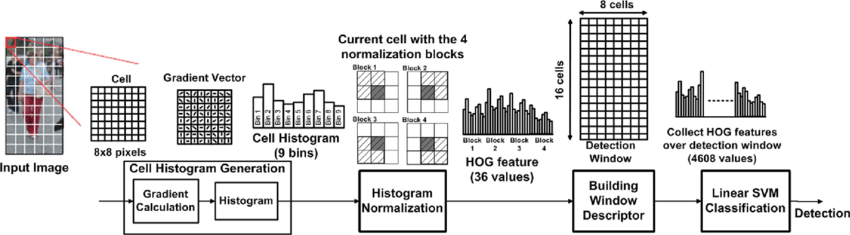
\includegraphics[width=\textwidth]{HOG-features.png}
\caption{Desde su pulicación para cada una de las etapas en la detecció de objetos, se han relizado propuestas de mejoras por ejemplo su implementación en sistemas embebidos \cite{energy-hog}}
\label{fig:hog}
\end{figure}



\subsection*{Generación de candidatos}
\subsubsection*{\textbf{Ventana deslizante}}
\begin{figure}[ht]
\centering
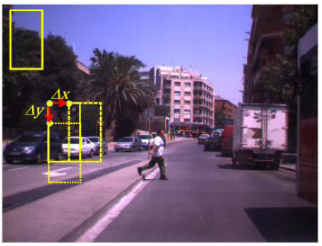
\includegraphics[width=8cm]{ventana.png}
\caption{\label{tab1}Ventana deslizante de tamaño 128x64 utilizada para la detección de peatones en [1].} 
\label{fig:ventana}
\end{figure}


\begin{algorithm}
\SetAlgoLined
\KwResult{Vector HOG para ventana}
 Dividir imagen en celdas 8x8\;
  \For {celdas en vertical} {
  calcular hog\;
  }
  \For{celdas en horizontal}{
  calcular hog\;
  }
  \While{Haya bloques por procesar}{
  crear bloque de 2x2 celdas\;
  crear HOG de bloque concatenado HOG de las 4 celdas\;
  Normalizar HOG de bloque\;
  }
  Crear HOG de la ventana concatendo HOG de los bloques
 \caption{Calculo de HOG para ventana}
\end{algorithm}



El procedimiento de ventana deslizante consiste en definir un rectángulo de dimensiones MxN e ir recorriendo la imagen.  Cada conjunto de píxeles (parte de la imagen) que se encuentren dentro de la ventana son extraídos y presentados como posibles  candidatos para localizar el objeto de nuestro interés que en este caso se trata de un rostro humano. 
El tamaño de la ventana debe tener la proporción del objeto a encontrar en la imagen. En [1] el tamaño con mejores resultados es de 128x64 píxeles debido a que es la proporción que determinaron para localizar un humano, en nuestro caso consideramos las proporciones de un rostro humano cuadrados y utilizaremos un a ventana de 80x80 píxeles.
\subsubsection*{\textbf{Pirámide de la imagen}}
Consiste en redimensionar la imagen para que la ventana de tamaño fijo que recorre la imagen durante la extracción de candidatos pueda captura el objeto a identificar, por ejemplo si una persona se encuentra en primer plano su rostro aparecerá con mayores dimensiones que el rostro de una persona que se encuentra al fondo. Si la ventana es de tamaño 80x80 píxeles y el rostro en primer plano es de tamaño 120x120 píxeles entonces no se detectará en el tamaño original de la imagen, pero si se detectará en la misma imagen con dimensiones 1/2 del original para tal caso el rostro en primer plano tendrá un tamaño de 60x60 píxeles. \\

\begin{figure}
\centering
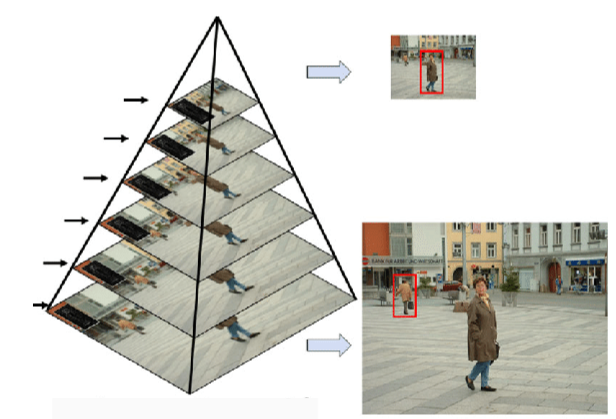
\includegraphics[width=8cm]{piramide-00.png}
\caption{La imagen es redimensioanda para que la ventana pueda capturar objetos mas grandes que el tamaño de la ventana}
\label{fig:piramide}
\end{figure}

\begin{figure}[ht]
\centering
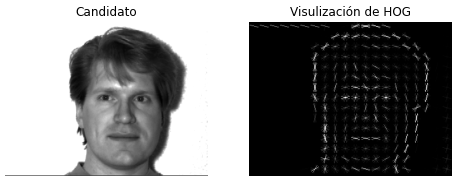
\includegraphics[width=10cm]{viz-hog.png}
\caption{En el lado izquierdo se muestra una imagen candidata y del lado derecho una visualización de su vector característico o HOG. La visualización del vector de características no forma parte del proceso de identificación del objeto. }
\label{fig:hog-viz}
\end{figure}

\section*{Clasificador lineal SVM}
Un modelo SVM es una representación de los vectores HOG como puntos en el espacio, mapeados de modo que los HOG que contienen un rostro humano queden separados por el margen más grande posible de aquellos que no. Luego, los nuevos HOG se mapean en ese mismo espacio y se predice a que categoría pertenecen según el lado del espacio que se les asigna. 

Para este paso de clasificación, Dalal y Triggs en [1] emplean una SVM "Support Vetor Machine"  para determinar si el descriptor HOG generado es mapeado en una de las clases predefinidas, peatón o no peatón. 

Un efecto secundario, benefico hasta cierto punto ya que confirma que el sistema funciona, son la detecciones de un mismo objeto en la image pero con diferentes candidatos superpuestos. La imagen \ref{fig:nms} muestra este caso. Para seleccionar un solo candidato como resultado de la detección del objeto se aplica un método llamado  \textbf{Non Maximum Supression} que eliminará otros candidatos que corresponden al mismo objeto.
\begin{figure}[ht]
\centering
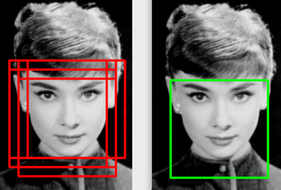
\includegraphics[width=.5\textwidth]{NMS.png}
\caption{El objetivo de un sistema detector de objetos es indicarnos su ubicación mediante las coordenadas dentro de la imagen , la evaluación de diferentes candidados por medio de la ventana deslizante tiene como efecto secundaro reportar la ubicación del mismo objeto pero en ventanas diferentes que se superponen. Del lado izquierdo vemos 6 ventanas que detectaron el mismo rostro en la imagen, en el lado derecho el resultado de aplicar el método de NMS. }
\label{fig:nms}
\end{figure}

\section*{Definición del problema a resolver}
Implementar un sistema de detección y reconocimiento  de objetos semi-rígidos, rostros humanos, utilizando HOG como descriptor o vector de características y una SVM como clasificador. 

El sistema completo leerá una imagen en escala de grises o rgb, por medio del método de ventanas deslizantes sobre la imagen a diferentes escalas se generarán candidatos que tendrán asociado un descriptor HOG, en una primera etapa este descriptor se evaluará en una SVM previamente entrenada y teniendo como resultado si el HOG corresponde a un rostro humano.  En una segunda etapa sí el HOG fue clasificado positivamente (la imagen asociada contiene un rostro) entonces se comparará con otros descriptores de rostros existentes en una base de datos para asociarla con un sujeto. Durante el desarrollo de la implementación se identificarán procedimientos que son susceptibles a una refactorización en otro lenguaje de programación  y/o  directivas de paralelismo.

\section*{Estrategía numérica}
\subsubsection*{Cálculos sobre las imágenes}
Se trabajara con las imágenes como arreglos \(2D\) si es en escala de grises, o arreglos \(3D\) en el caso de imágenes a color. Para llevar a cabo las diferentes operaciones a nivel de píxel será necesario cambiar el tipo de variables de entero sin signo de 8 bits a punto flotante de 32 bits.

\begin{figure}[ht]
\centering
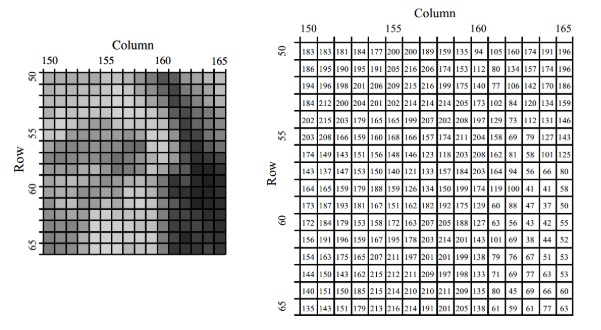
\includegraphics[width=.75\textwidth]{imagen-matriz.jpg}
\caption{Para una imagen en escala de grises  cada pixel representa la intensidad en el rango [0,255], estos calores puede ser representados una variable entera sin signo de 8 bits. }
\label{fig:imagen-matriz}
\end{figure}


\subsection*{Descriptor HOG}
El descriptor  histograma de gradientes orientados se obtendrá para los candidatos según la propuesta de \cite{dalal-triggs} con las variantes: celdas de tamaño 8x8, y  bloques 2x2,    recordando que estos candidatos son partes o pedazos de la imagen de tamaño 80x80 píxeles dando como resultado 10 celdas en la horizontal y vertical. El histograma tendrá 9 clases sobre el rango de 0 a 180 grados para los ángulos de los gradientes distribuyendo las magnitudes con interpolación bilineal dentro de las celdas y trilinear en los bloques. El tamaño del vector HOG sera de \(9 * 9 * 4 * 9 = 2916\)

\subsection*{Diferencial de la imagen}
Se calcula de forma horizontal (y) y vertical (x) y consiste en asignar a cada píxel el resultado de restar el valor del píxel previo al valor del píxel posterior:

\begin{lstlisting}[language=C, caption=Calculo de la imagen diferencial]
//diferencial horizontal
for y=1; y<80 ;y++
 for x=1; x<80: x++
  dif_x[y][x] = img[y][x+1] - img[y][x-1]
//diferencial vertical
for x=1; y<80 ;y++
 for y=1; x<80: x++
  dif_y[y][x] = img[y+1][x] - img[y-1][x]  

\end{lstlisting}
Debido a que estas operaciones son independientes, es decir el cálculo sobre un píxel no es dependencia del cálculo de otro, de pueden llevar a cabo de forma paralela.

\subsection*{Magnitud y dirección del gradiente}
Con las diferenciales sobre la horizontal y vertical el siguiente paso es calcular la magnitud y dirección del gradiente asociado a cada píxel. 

\begin{lstlisting}[language=C, caption=Calculo de la imagen magnitud y direcciones]
for y=1; y<80 ;y++
 for x=1; x<80: x++
  temp = dif_y[y][x]*dif_y[y][x] +
         dif_x[y][x]*dif_x[y][x]
  mag[y][x] = sqrt(temp)

for y=1; y<80 ;y++
 for x=1; x<80: x++
  temp2 = arctan(dif_x[y][x]/dif_y[y][x])
  if temp2 < 0 ; temp2 = temp2 * -1 
  dir[y][x] = temp2 * (180/\pi})

\end{lstlisting}

Se puede observar que las operaciones para las magnitudes y ángulos o direcciones de los gradientes se puede llevar a cabo de forma paralela debido a que todas las operaciones son independientes 

\subsection*{Construcción del histograma}
En el desarrollo del \cite{dalal-triggs} se reportan la construcción del histograma tomando como valores de la clase segmentos de ángulo en el rango [0-180] grados, con tamaños de clase desde 10 (18 clases) y hasta 60 grados (3 clases). El número de clases con el que se reportan mejores resultados es de 9 (tamaño de clase 20 grados). \\

Para construir el histograma de una celda de 8x8 píxeles se enumeran las 9 clases de 0..8 con un ancho cada una de 180/20=20 grados.  Cada magnitud será distribuido entre las 2 clases mas cercanas al ángulo asociado al píxel mediante un factor de peso que será calcula a partir de la distancia al punto medio de  las clases que delimitan al ángulo.\\ 
Por ejemplo para distribuir la magnitud U cuyo ángulo es 77 grados, las 2 clases que lo delimitan son la clase 3:[60-80) y la clase 4:[80-100), la distancia entre los puntos de medios de ambas clases son (80+20)/2-77=13 y 77-(60+20/2)=7.  Los pesos para distribuir la magnitud del gradiente serán:  13/20 = 0.65 para la clase 3 y 1-0.65=0.35 para la clase 4. 

\begin{lstlisting}[language=C, caption=Calculo de la imagen diferencial]

for y=1; y<80 ;y++
 for x=1; x<80: x++
  ang = dir[y][x]
  clas_i = flor(ang/20)
  clas_s = clas_i + 1
  pm_clas_i = (clas_i*20)+20/2
  pm_clas_s = pm_clas_i + 20
  dist_pm_clas_i = abs(pm_clas_i - ang )
  dist_pm_clas_s = abs(pm_clas_s - ang )
  fact_clas_i = (1 - dist_pm_clas_i)/20
  fact_clas_s = (1 - dist_pm_clas_s)/20

\end{lstlisting}

El siguiente paso es agrupar bloques de 2x2 celdas y concatenar los 4 histogramas y aplicar una normalización L2 sobre los 36 elementos resultantes. La agrupación de bloques debe ser de tal forma que se encimen en una celda por la vertical y la horizontal, esquema  semejante al de ventana deslizante. Para nuestro caso con una imagen candidato de tamaño 80x80 tenemos 10 celdas por la horizontal y al realizar el agrupamiento tipo ventana deslizante generaremos 9 bloques que corresponden a 9 histogramas normalizados y lo mismo para la vertical. Estos 81 histogramas se concatenan y vuelven a normalizados.  El descriptor HOG así obtenido para nuestro candidato es un vector de longitud 81x36=2916.


\section*{Discusión}
El procesamiento de imágenes para la extracción de HOG tiene varios procesos que son susceptibles a una implementación en paralelo podemos mencionar el cálculo de la imagen diferencial, la imagen de magnitudes y la  imagen de orientaciones o de ángulos.  Por otro lado es posible procesar cada uno de los candidatos obtenidos mediante la pirámide de imágenes de forma independiente así como la clasificación del descriptor HOG mediante el uso de la SVM.\\

Un primer paso para explorar la implementación de las diferentes etapas para la detección y reconocimiento  de rostros humanos es utilizando el lenguaje de programación python\cite{pythonwebsite} y de paquetes auxiliares para el tratamiento de matrices que no permitirán realizar un prototipo que nos permite identificar elementos susceptibles a ser paralelizados o refactorizados para un mejor desempeño.\\

El paquete utilizado fue numpy\cite{numpywebsite}. El funcionamiento de numpy se basa en el objeto ndarray (N-dimencional array) el cual permite realizar distintas operaciones sobre los elemento de un arreglo. Si partimos del hecho que una imagen es un arreglo 3D, en caso de una imagen a color con los canales  R,G,B; o 2D como es caso de una imagen en escala de grises, diferentes procedimientos que se deben aplicar a una imagen para durante el proceso de reconocimiento de rostros se llevan cabo en un par de líneas de código utilizando numpy. \\

Por ejemplo. Sea imagen un arreglo numpy NxM que contiene el candidato procesar, sean gy y gx dos arreglos del mismo tamaño que el arreglo imagen, entonces podemos realizar la imagen diferencial con las siguientes 2 líneas:

\begin{lstlisting}[language=python, caption=Calculo de la imagen diferencial]
gy[1:-1,:]  = imagen[2:,:]-imagen[0:-2,:]
gx[:,1:-1]  = imagen[:,2:]-imagen[:,0:-2]
\end{lstlisting}

Otros ejemplos del uso de numpy con el calculo de la imagen de magnitudes y la imagen de direcciones o ángulos de la imagen gradiente

\begin{lstlisting}[language=python, caption=Calculo de la imagen diferencial]
mag = np.sqrt(gx**2 + gy**2)
ang = (np.arctan2(grx, gry)*(180/np.pi))
ang = np.where(ang< 0,-ang,ang)
\end{lstlisting}




\begin{thebibliography}{11}
\bibitem{placas} 
Lubna, M. F. Khan and N. Mufti, "Comparison of various edge detection filters for ANPR," 2016 Sixth International Conference on Innovative Computing Technology (INTECH), Dublin, 2016, pp. 306-309, doi: 10.1109/INTECH.2016.7845061.
Michel Goossens, Frank Mittelbach, and Alexander Samarin. 

\bibitem{dalal-triggs}
Navneet Dalal, Bill Triggs.  Histograms of Oriented Gradients for Human Detection.  InternationalConference on Computer Vision and Pattern Recognition (CVPR ’05), Jun 2005, San Diego, UnitedStates. pp.886–893, 10.1109/CVPR.2005.177. inria-00548512

\bibitem{hog-parts1}
A Discriminatively Trained, Multiscale, Deformable Part Model
P. Felzenszwalb, D. McAllester, D. Ramanan
IEEE Conference on Computer Vision and Pattern Recognition (CVPR), 2008 

\bibitem{hog-parts2}
P. Felzenszwalb, R. Girshick, D. McAllester, D. Ramanan
IEEE Transactions on Pattern Analysis and Machine Intelligence, Vol. 32, No. 9, September 2010 

\bibitem{viola-jones}
P. Viola and M. Jones, "Robust real-time face detection," Proceedings Eighth IEEE International Conference on Computer Vision. ICCV 2001, Vancouver, BC, Canada, 2001, pp. 747-747, doi: 10.1109/ICCV.2001.937709.

\bibitem{caras-resumen}
Yang, Ming-Hsuan and Kriegman, David and Ahuja, Narendra. (2002). Detecting Faces in Images: A Survey. Pattern Analysis and Machine Intelligence, IEEE Transactions on. 24. 34 - 58. 10.1109/34.982883. 

\bibitem{energy-hog}
Suleiman, Amr and Sze, Vivienne. (2016). An Energy-Efficient Hardware Implementation of HOG-Based Object Detection at 1080HD 60 fps with Multi-Scale Support. Journal of Signal Processing Systems. 84. 10.1007/s11265-015-1080-7. 

\bibitem{pythonwebsite}
Python is a programming language that lets you work more quickly and integrate your systems more effectively.
\\\texttt{https://www.python.org/}

\bibitem{numpywebsite}
The fundamental package for scientific computing with Python
\\\texttt{https://numpy.org/}

\bibitem{scikitwebsite}
Scikit-learn is an open source machine learning library that supports supervised and unsupervised learning. 
\\\texttt{https://scikit-learn.org/}

\end{thebibliography}

\end{document}
